% MIT License

% Copyright (c) 2022 Chiyuru

% Permission is hereby granted, free of charge, to any person obtaining a copy of this software and associated documentation files (the "Software"), 
% to deal in the Software without restriction, including without limitation the rights
% to use, copy, modify, merge, publish, distribute, sublicense, and/or sell
% copies of the Software, and to permit persons to whom the Software is
% furnished to do so, subject to the following conditions:

% The above copyright notice and this permission notice shall be included in all copies or substantial portions of the Software.

% THE SOFTWARE IS PROVIDED "AS IS", WITHOUT WARRANTY OF ANY KIND, EXPRESS OR IMPLIED, INCLUDING BUT NOT LIMITED TO THE WARRANTIES OF MERCHANTABILITY,
% FITNESS FOR A PARTICULAR PURPOSE AND NONINFRINGEMENT. IN NO EVENT SHALL THE AUTHORS OR COPYRIGHT HOLDERS BE LIABLE FOR ANY CLAIM, DAMAGES OR OTHER
% LIABILITY, WHETHER IN AN ACTION OF CONTRACT, TORT OR OTHERWISE, ARISING FROM,
% OUT OF OR IN CONNECTION WITH THE SOFTWARE OR THE USE OR OTHER DEALINGS IN THE SOFTWARE.

% Define the command to use the bold symbol in math environment
\newcommand{\mb}[1]{\boldsymbol{#1}}

\documentclass[UTF8]{ctexart}

\usepackage{amsmath}
\usepackage{cases}
\usepackage{cite}
\usepackage{graphicx}
\usepackage[margin=1in]{geometry}
\geometry{a4paper}
\usepackage{fancyhdr}
\pagestyle{fancy}
\fancyhf{}

\title{孤立系统中单管引水的水轮机调节系统\\小波动特性分析报告}
\author{刘锦坤}
\date{}

\pagenumbering{arabic}

\begin{document}

\fancyhead[C]{波动特性分析报告}
\fancyfoot[C]{\thepage}

\maketitle
\tableofcontents

\section{说明}

本次作业所有文件均已上传至附件,代码保存在code文件夹,图片保存在pic文件夹,问题[n]对应的代码为Question[n].py文件,util.py文件为编写的工具函数文件,其中包括了若干矩阵运算函数。运行python程序前请确保

\begin{enumerate}
  \item 安装了python3.7及以上版本,实地测试环境为python3.11.4
  \item 安装了符合python版本的numpy, matplotlib, scipy, tkindter等python库
  \item 保证util.py文件与Question[n].py文件在同一目录下
\end{enumerate}

\section{问题一}

运行Question1.py文件,即可打印出AR矩阵元素和转移矩阵的元素:

\begin{verbatim}
    Matrix A_R is:
[[ -0.223        0.076        0.           0.1665      -0.1       ]
 [-10.          -0.4        -10.           0.           0.        ]
 [ -8.          -0.32        -8.2          0.           0.        ]
 [ 13.26435742   0.57419531  13.37890625  -0.54986471  -0.05136719]
 [  0.           0.           0.           0.           0.        ]]
    The transition matrix is:
[[ 9.92406723e-01  2.95483905e-03  9.61190807e-04  6.31148589e-03
  -3.83722343e-03]
 [-3.27432401e-01  9.86337929e-01 -3.27586450e-01 -1.09813331e-03
   6.65067258e-04]
 [-2.60885797e-01 -1.08860649e-02  7.31328490e-01 -8.76193562e-04
   5.30655930e-04]
 [ 4.28617119e-01  1.95475459e-02  4.33162394e-01  9.80517570e-01
  -2.82955859e-03]
 [ 0.00000000e+00  0.00000000e+00  0.00000000e+00  0.00000000e+00
   1.00000000e+00]]
\end{verbatim}

同时绘制出转速$n$的过渡过程曲线如图1所示,可以看到,在经过一段时间后,转速$n$会进入一个新的稳定值。

\begin{figure}[htbp]
    \centering
    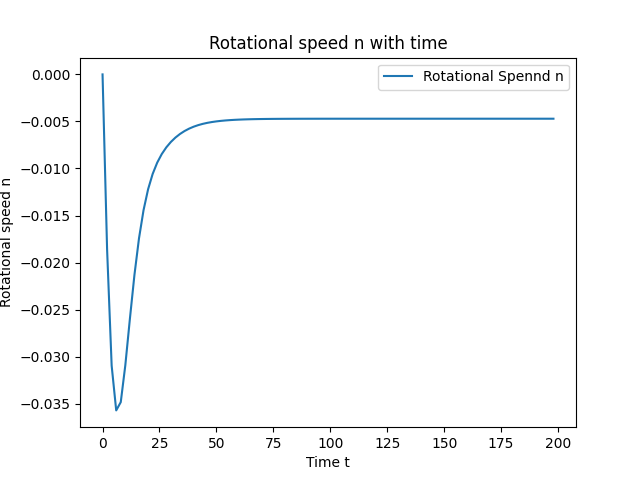
\includegraphics[width=0.8\textwidth]{pic/n-t.png}
    \caption{转速$n$的过渡过程曲线}
\end{figure}

\section{问题二}

运行Question2.py文件,即可得到不同的$T_d,b_t$的值对应的过渡过程曲线如图2所示:

\begin{figure}[htbp]
    \centering
    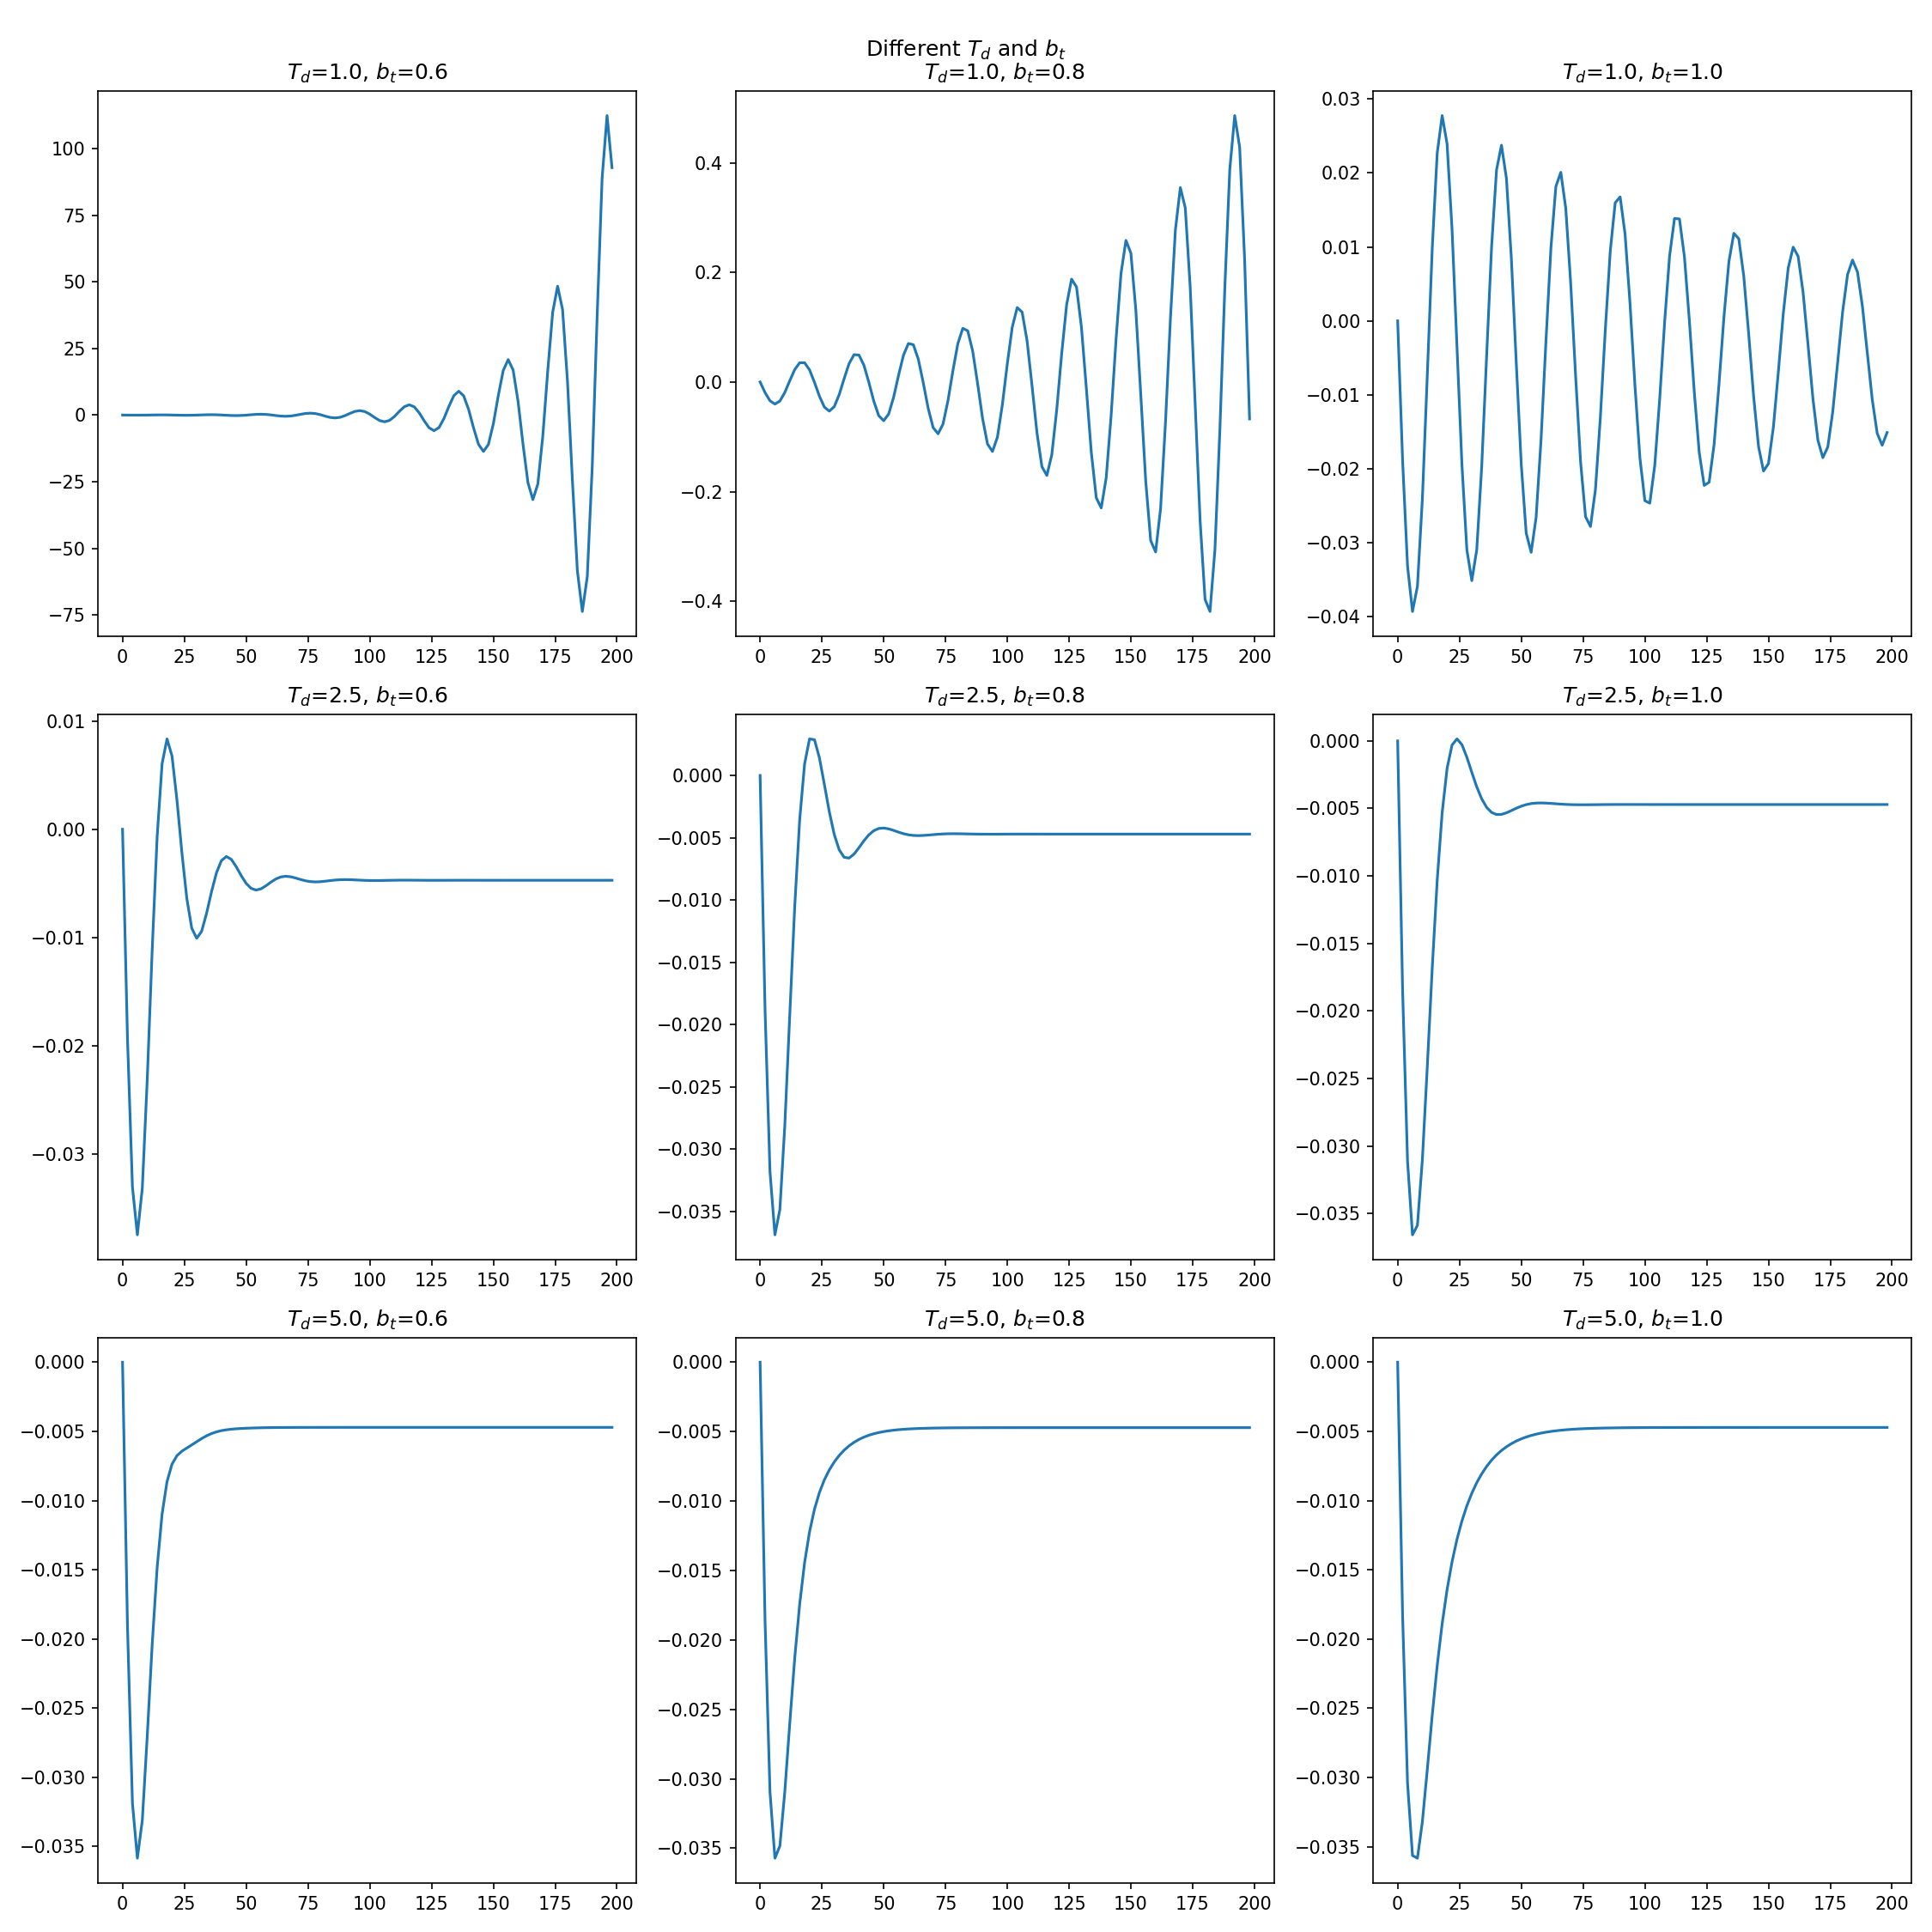
\includegraphics[width=0.8\textwidth]{pic/dif_td_bt.png}
    \caption{$T_d,b_t$的不同值对应的过渡过程曲线}
\end{figure}

可以看到,在$T_d$和$b_t$都较小时,系统在扰动后偏离平衡态,在扰动下不稳定。而$b_t$增大后,系统再次进入稳定域,说明$b_t$的增大有助于系统的稳定。同时还能发现,在一定范围内$T_d$和$b_t$的增大都能减少系统的超调,提高系统的动态品质。

\section{问题三}

运行Question3.py文件,即可得到不同的$T_a$的值对应的过渡过程曲线如图3所示:

\begin{figure}[htbp]
    \centering
    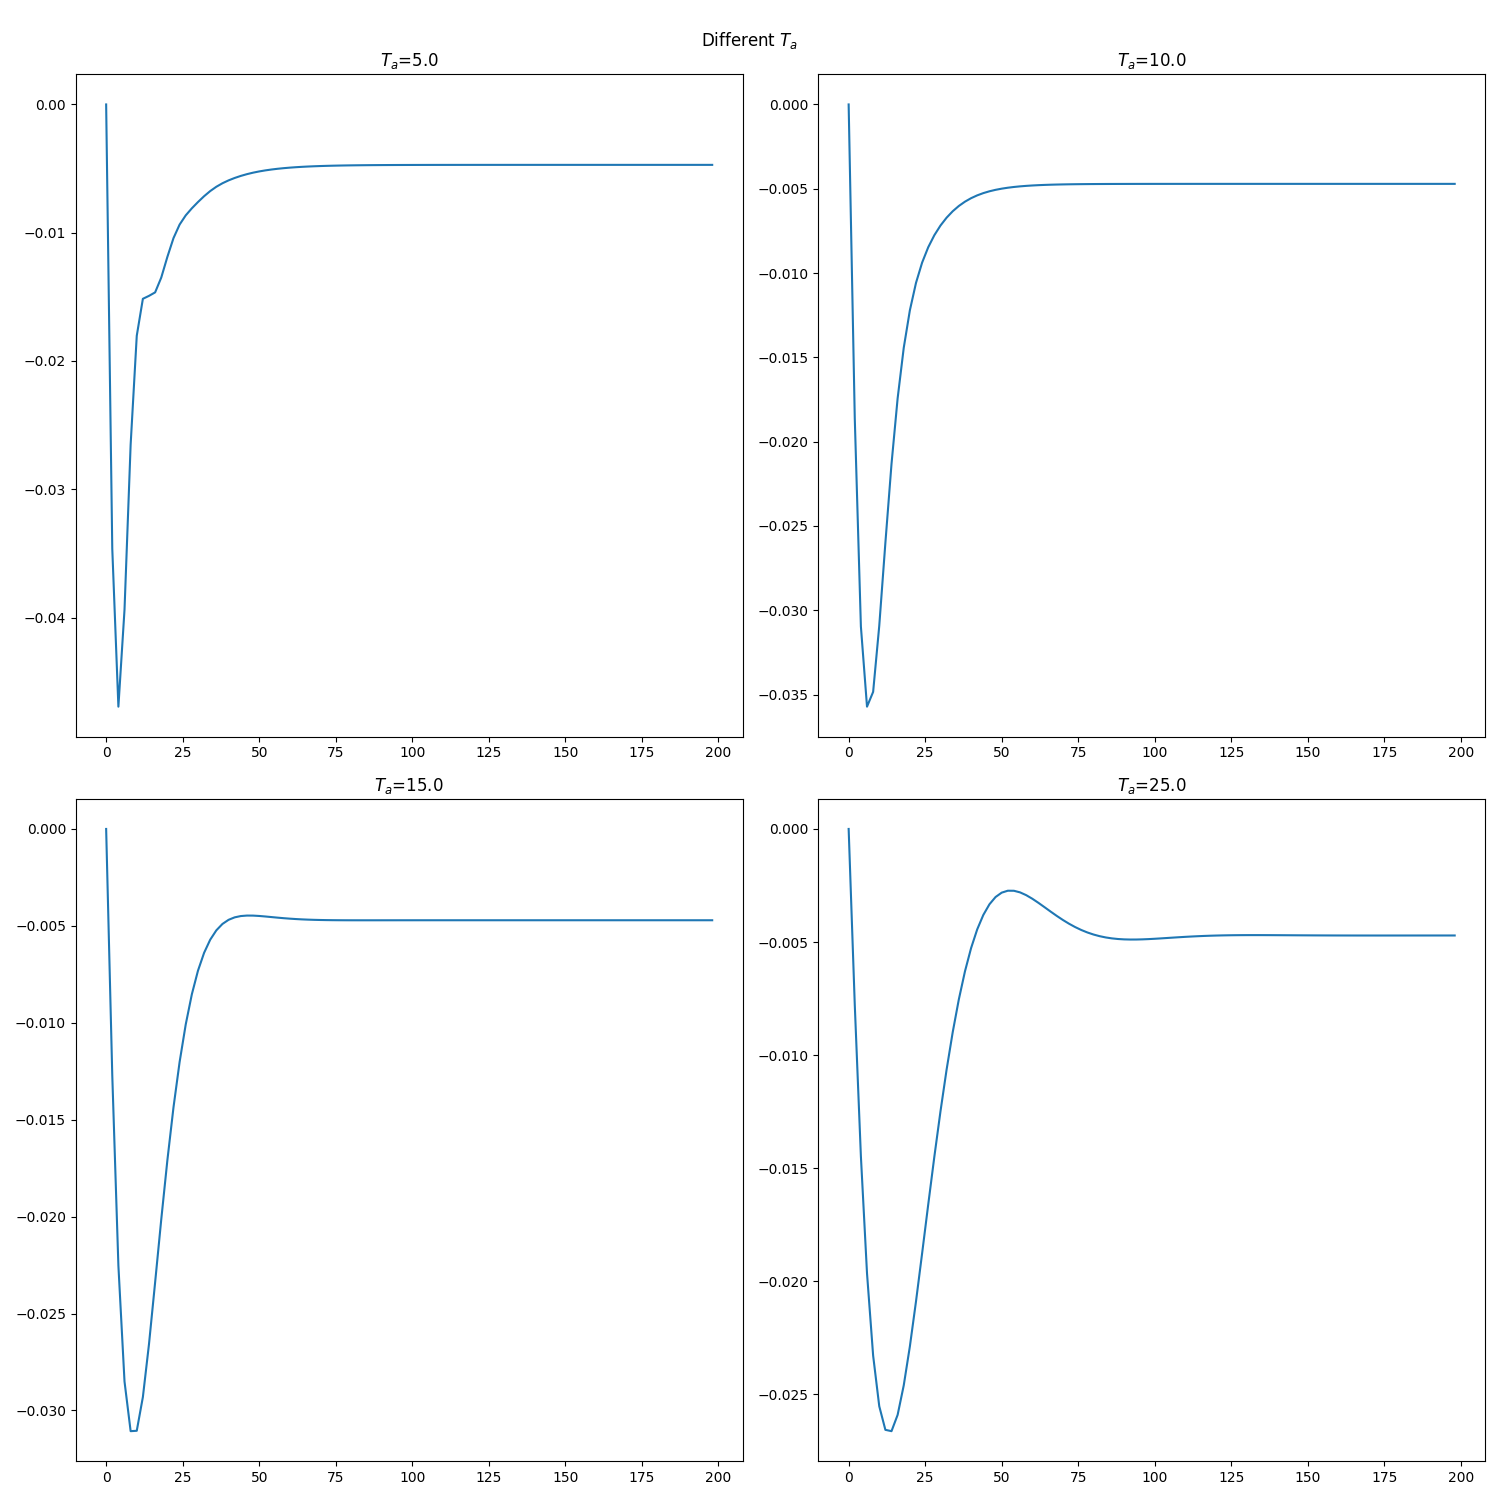
\includegraphics[width=0.8\textwidth]{pic/dif_ta.png}
    \caption{$T_a$的不同值对应的过渡过程曲线}
\end{figure}

可以看到,$T_a$的增大会使得系统的超调量增大,调节时间变长,因此在一定范围内$T_a$的增大会使得系统的动态品质变差,但是由于超调量的增大,系统的稳定性很可能会增强。

\section{问题四}

运行Question4.py文件,即可得到不同的$T_w$的值对应的过渡过程曲线如图4所示:

\begin{figure}[htbp]
    \centering
    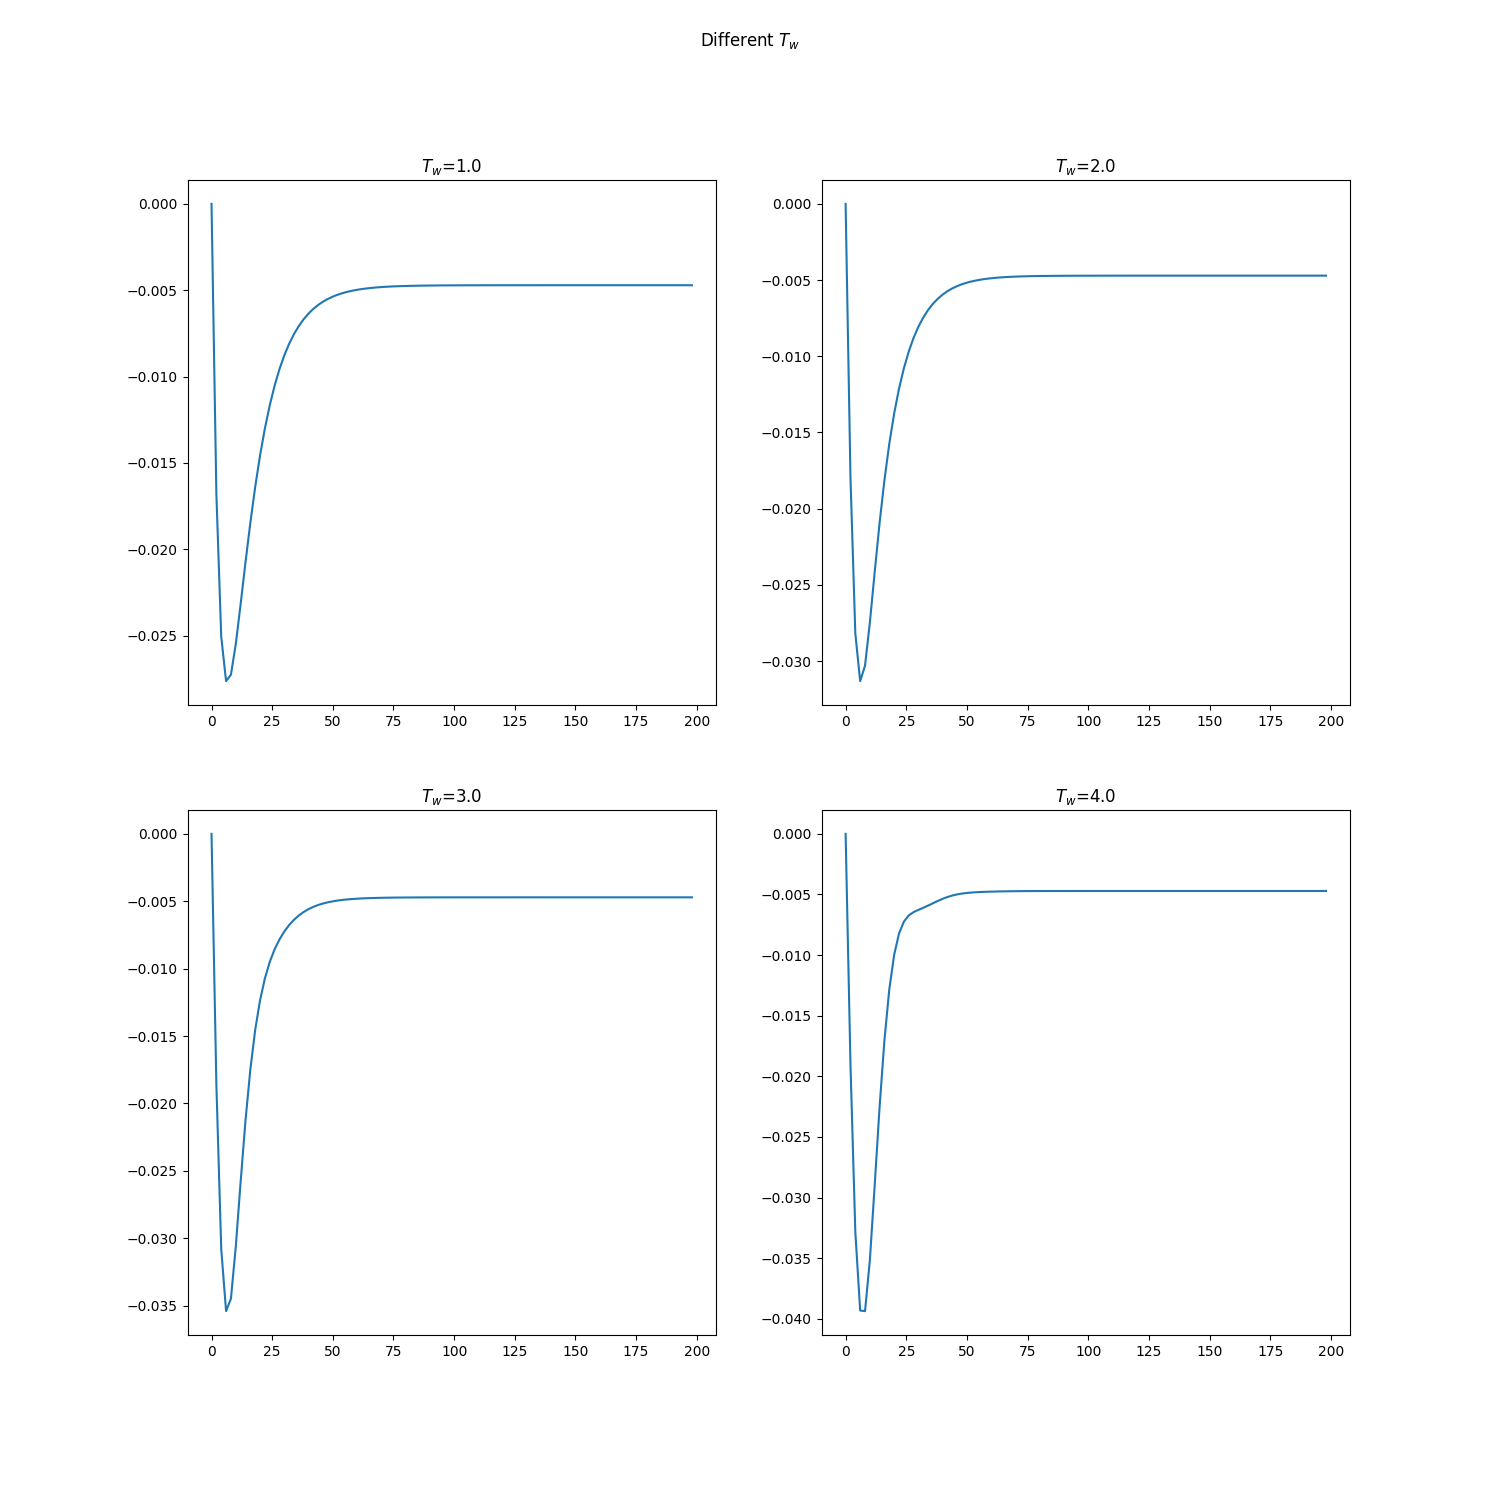
\includegraphics[width=0.8\textwidth]{pic/dif_tw.png}
    \caption{$T_w$的不同值对应的过渡过程曲线}
\end{figure}

可以看到,更大的$T_w$会使得系统向下的振荡幅度更大,因此在一定范围内$T_w$的增大会使得系统的动态品质变差,也可能会使得系统的稳定性变差。

\section{问题五}

这里我们可以进行一个理论推导分析系统的稳定性,对于矩阵方程

\begin{equation}
  \mb{\dot x} = \mb A \mb x
\end{equation}

其解为

\begin{equation}
  \mb x = \mb x_0 e^{\mb A t}
\end{equation}

而该解要是渐近稳定的(即不发散),则要求对于矩阵$\mb A$的所有特征值$\lambda_i$均满足实部小于0的条件,即

\begin{equation}
  \text{Re}(\lambda_i) < 0  
\end{equation}

那么对于一组特定的特定的传递系数,我们只需计算矩阵$\mb A_R$的特征值即可判断系统的稳定性。在Question5.py文件中,我们实现了对于不同传递系数计算矩阵$\mb A_R$的特征值,并且绘制转速曲线代码。可以通过滑块自由变动传递系数,观察特征值的变化和系统的稳定性,如图5所示。

\begin{figure}[htbp]
    \centering
    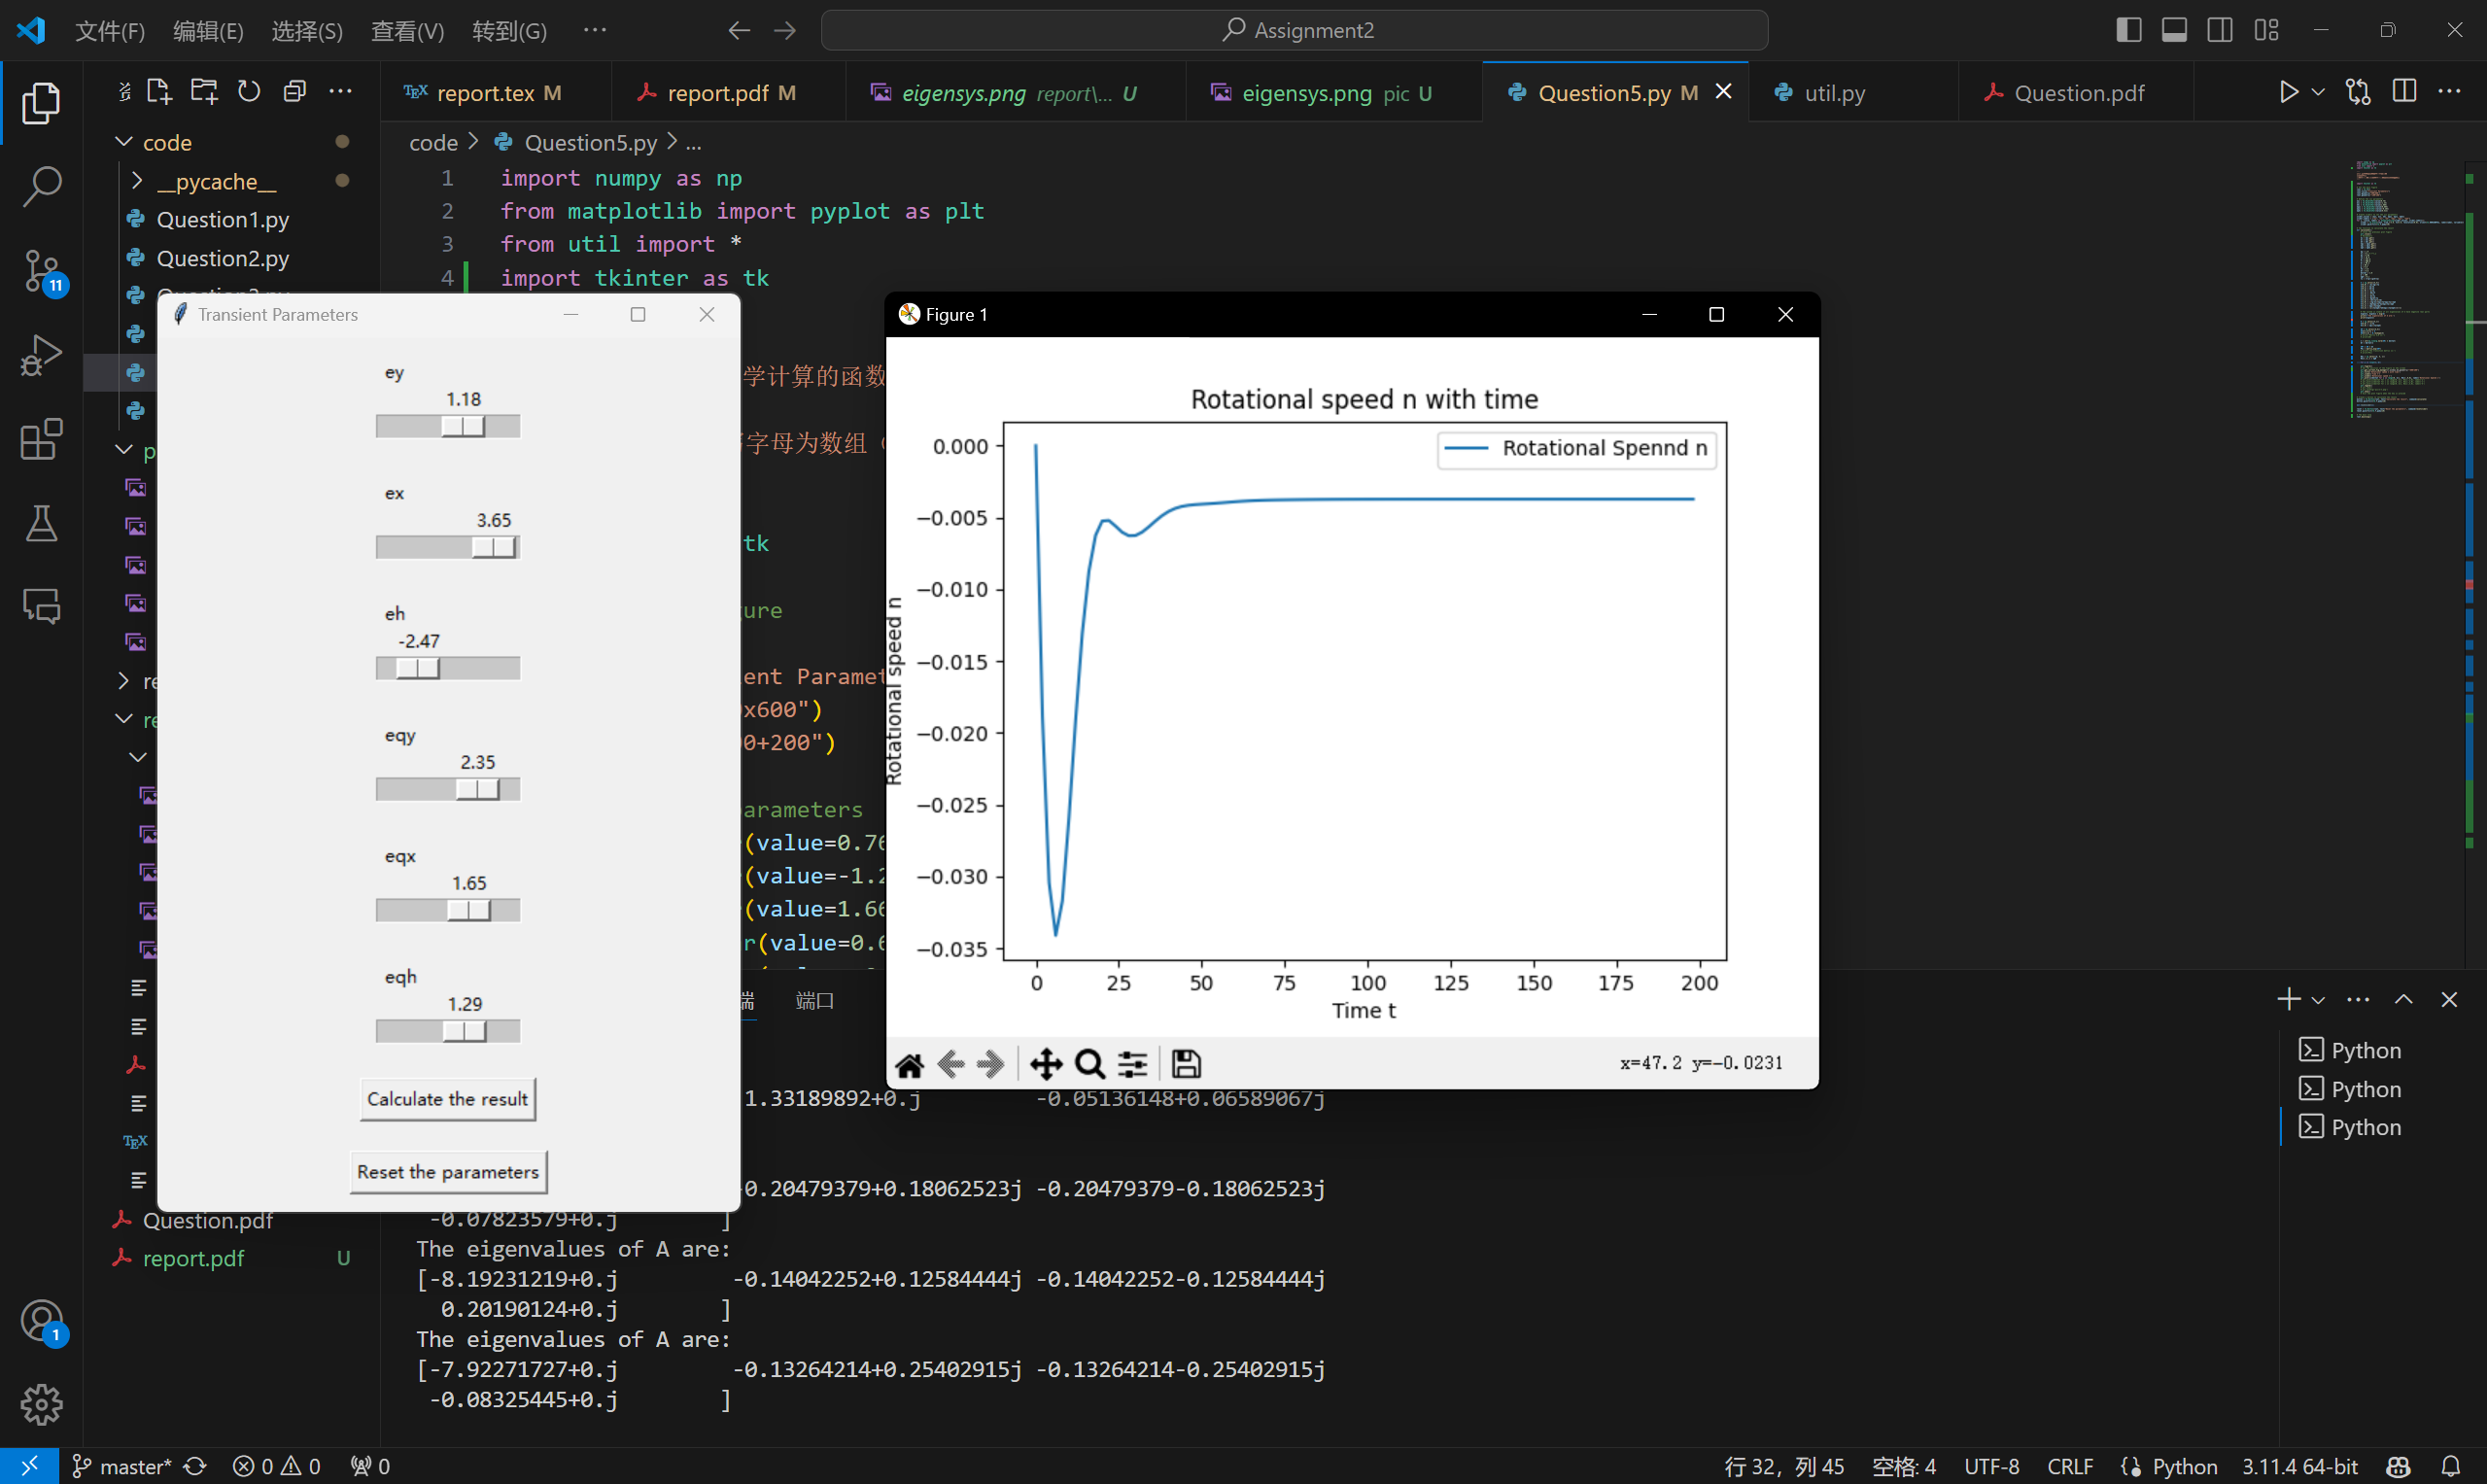
\includegraphics[width=0.8\textwidth]{pic/eigensys.png}
    \caption{特征值的变化}
\end{figure}

最终会发现当传递系数在一定范围内时,当使得矩阵$\mb A_R$的特征值的实部全为负时,系统是稳定的,而当传递系数超出一定范围时,矩阵$\mb A_R$的特征值的实部出现正数(或0),系统会变得不稳定。具体对于每一个传递系数来说:

\begin{enumerate}
  \item $e_y$增大时系统向平衡稳定方向偏离,减小时向不平衡方向偏离。
  \item $e_x$增大时系统向不平衡稳定方向偏离,减小时向平衡方向偏离。
  \item $e_h$增大时系统向不平衡稳定方向偏离,减小时向平衡方向偏离。
  \item $e_{qy}$增大时系统向不平衡稳定方向偏离,减小时向平衡方向偏离。
  \item $e_{qx}$增大时系统向平衡稳定方向偏离,减小时向不平衡方向偏离。
  \item $e_{qh}$增大时系统向平衡稳定方向偏离,减小时向不平衡方向偏离。
\end{enumerate}

\end{document}

